\documentclass[10pt,twocolumn]{witseiepaper}

\usepackage{KJN}
\usepackage{chngcntr}
\usepackage{multicol}

\ifpdf
\pdfinfo{
/Title (ELEN4012 - Feature Based Automatic Modulation Classification)
/Author (Jacques Visser and Anthony Farquharson)
}
\fi

\begin{document}

\title{ELEN4012 - Feature Based Automatic Modulation Classification}

\author{Anthony Farquharson and Jacques Visser
\thanks{School of Electrical \& Information Engineering, University of the
Witwatersrand, Private Bag 3, 2050, Johannesburg, South Africa}
}

% TODO Rewrite abstract once the rest of the contents are figured out.
\abstract{Abstract!}

\keywords{modulation, classification, USRP, UHD}

\maketitle
\thispagestyle{empty}\pagestyle{empty}

% TODO How does one even write an introduction?
\section{INTRODUCTION}

\section{LITERATURE SURVEY}
\label{sec:literature}
According to Zhu and Nandi \cite{zhu2014automatic} there are three primary approaches to automatic modulation classification (AMC), these are: likelyhood-based, distribution-test-based and feature based. These will be discussed briefly below.

	\subsection{Likelihood Based Classification}
	\label{subsec:likelyhood}
	Likelihood based classification is the considered the most popular method of classification, due to the accuracy of the classification when the channel is perfectly modeled \cite{zhu2014automatic}. This method requires knowledge of the channel that the signal is received from, which can be derived through evaluating every modulation hypothesis with observed signal samples \cite{zhu2014automatic}.\\[11pt]

	The main likelihood based classifier approaches are as follows \cite{zhu2014automatic}:
	\begin{itemize}
		\item \textbf{Maximum Likelihood (ML)} - This classifier requires perfect channel knowledge and all parameters are known except for the signal modulation.
		\item \textbf{Average Likelihood Ratio Test (ALRT)} - This classifier overcomes the limitation of not knowing every parameter through using accurate models for unknown parameters, making the calculation much more complex when unknown parameters are introduced.
		\item \textbf{Generalized Likelihood Ratio Test (GLRT)} - Essentially a combination of ALRT and ML classifiers, it replaces the integration of unknown parameters (ALRT) with maximization of likelihood for a possible range of unknown parameters.
		\item \textbf{Hybrid Likelihood Ratio Test (HLRT)} - The HLRT likelihood function is calculated by averaging transmitted symbols and maximizing the resulting function.
	\end{itemize}
	These classifiers are well documented by Zhu and Nandi \cite{zhu2014automatic}; and Dobre, Abdi, Bar-Ness and Su \cite{dobre2007survey}. 

	\subsection{Distribution Test Based Classification}
	\label{subsec:distribution}
	
	The distribution test based classification uses the symbol mapping, which is associated with a particular modulation scheme. This is assuming that the channel parameters are pre-estimated and available \cite{zhu2014automatic}.
	
	The technique uses a method known as ``Goodness of Fit'' which will equate the differences between known signal cumulative distributions and the received signal cumulative distribution. The classification is completed by finding the signal distribution with the best goodness of fit \cite{zhu2014automatic}.
	
	There are many distribution tests which can be used to evaluate the goodness of fit, some of them are given below \cite{zhu2014automatic}:
	\begin{itemize}
		\item \textbf{Kolmogorov-Smirnov Test Classifier} - This goodness of fit test evaluates the equality of two probability distributions, for the classifier the sampled cumulative distribution function (CDF) and a hypothesized CDF are considered.
		\item \textbf{Cramer-Von Mises Test Classifier} - The method of the classifier is the same as the Kolmogorov-Smirnov classifier, but the goodness of fit criterion is different.
		\item \textbf{Anderson-Darling Test Classifier} - This classifier uses a weighted version of the Cramer-Von Mises test classifier. The tail of the distribution is weighted to counter the fact that it converges to zero at that point.
	\end{itemize}
	The distribution test based classifiers are well documented by Zhu and Nandi \cite{zhu2014automatic}; and Dobre, Abdi, Bar-Ness and Su \cite{dobre2007survey}.

	\subsection{Feature Based Classification}
	\label{subsec:feature}
	
	The feature based modulation classification is shown to not be as accurate, but is significantly less computationally intensive than the Distribution test based and likelihood based classifiers \cite{zhu2014automatic}.
	
	The feature based classification technique uses the primary features of a signal in order to classify it as a particular modulation scheme. The features that are primarily used to identify the signal vary depending on the method employed.
	
	The main methods of feature based classification are as follows \cite{zhu2014automatic}: 
	\begin{itemize}
		\item \textbf{Signal Spectral-Based Features} - The key features of a signal analyzed by this technique exploit the three primary signal aspects, namely the amplitude, phase and frequency. This technique is well documented by Azzouz and Nandi \cite{azzouz2013automatic}.
		\item \textbf{Wavelet Transform-based Features} - This classification technique uses a continues wavelet transform of a received signal in order to determine the type of modulation used, using known criterion for various modulation features.
		\item \textbf{High-order Statistics-based Features} - The statistics based classification technique can use moment based and cumulative based features in order to determine which modulation scheme is used on the signal.
	\end{itemize}
	The distribution test based classifiers are well documented by Zhu and Nandi \cite{zhu2014automatic}; Azzouz and Nandi \cite{azzouz2013automatic}; and Dobre, Abdi, Bar-Ness and Su \cite{dobre2007survey}.

\section{EXISTING SOLUTIONS AND APPLICATIONS OF AMC}
	\subsection{Military}
		% jamming, listening in on communications
	\subsection{Civilian}
		% cognitive radio, effective use of bandwidth
		% aircraft monitoring

\section{SOLUTION SELECTION}


\section{DESIGN PROCESS OVERVIEW}
	Automated modulation classification is primarily a software orientated problem, therefore a good development methodology must be laid out. In order to ensure quality of software output the following development methodologies are used.
	\subsection{Development Methodology}
	The development methodology chosen for this project is the Incremental Model, this model allows for a continuous use of small waterfall type development cycles \cite{incremental_model}. This methodology is chosen because the waterfall cycles allow for every iteration to be tested and integrated into the main project, reducing the chances of errors. \\[11pt]
	In order to track the various incremental cycles a Kanban approach \cite{kanban_model} will be used, this method uses a ``billboard'' of tasks, each task on the board will make up a small waterfall development cycle. These tasks will be tracked through use of Trello \cite{trello}, and every task will go through the stages from ``Pending'' to ``In Progress'' and finally ``Completed''.	

\section{IMPLEMENTATION OVERVIEW}
	\subsection{Hardware}
		The implementation will use a software defined radio, specifically the Universal Software Radio Peripheral (USRP) from Ettus Research \cite{ettus}. The USRP Hardware Driver (UHD) interfaces the software with the hardware system, due to lack of support for Windows this means the development will be done on Linux platforms.

	\subsection{Software}
	The UHD has an application programming interface (API) for use with the C++ programming language, allowing the development to be done in C++.
		\subsubsection{Basic Software Structure}
			As the algorithm should be ideally running in a real-time situation, the efficiency becomes a priority. For this reason the program will be threaded to allow for concurrent processes, this means that every major component will run on it's own thread.\\[11pt]
			The algorithm will separate the various processes out into their categories, allowing for a good layer separation. This means that components can be individually modified, replaced or mocked for testing. The program will run around a primary control loop, where information will be read from the UHD buffer, then processed (see Figure \ref{fig:sw_overview} below) and finally displayed. The feature extraction component is fully explored in Section \ref{subsec:feature_extract} below, and a full layout is given in Figure \ref{} in Appendix \ref{}.
			\begin{figure}[h!]
				\centering
				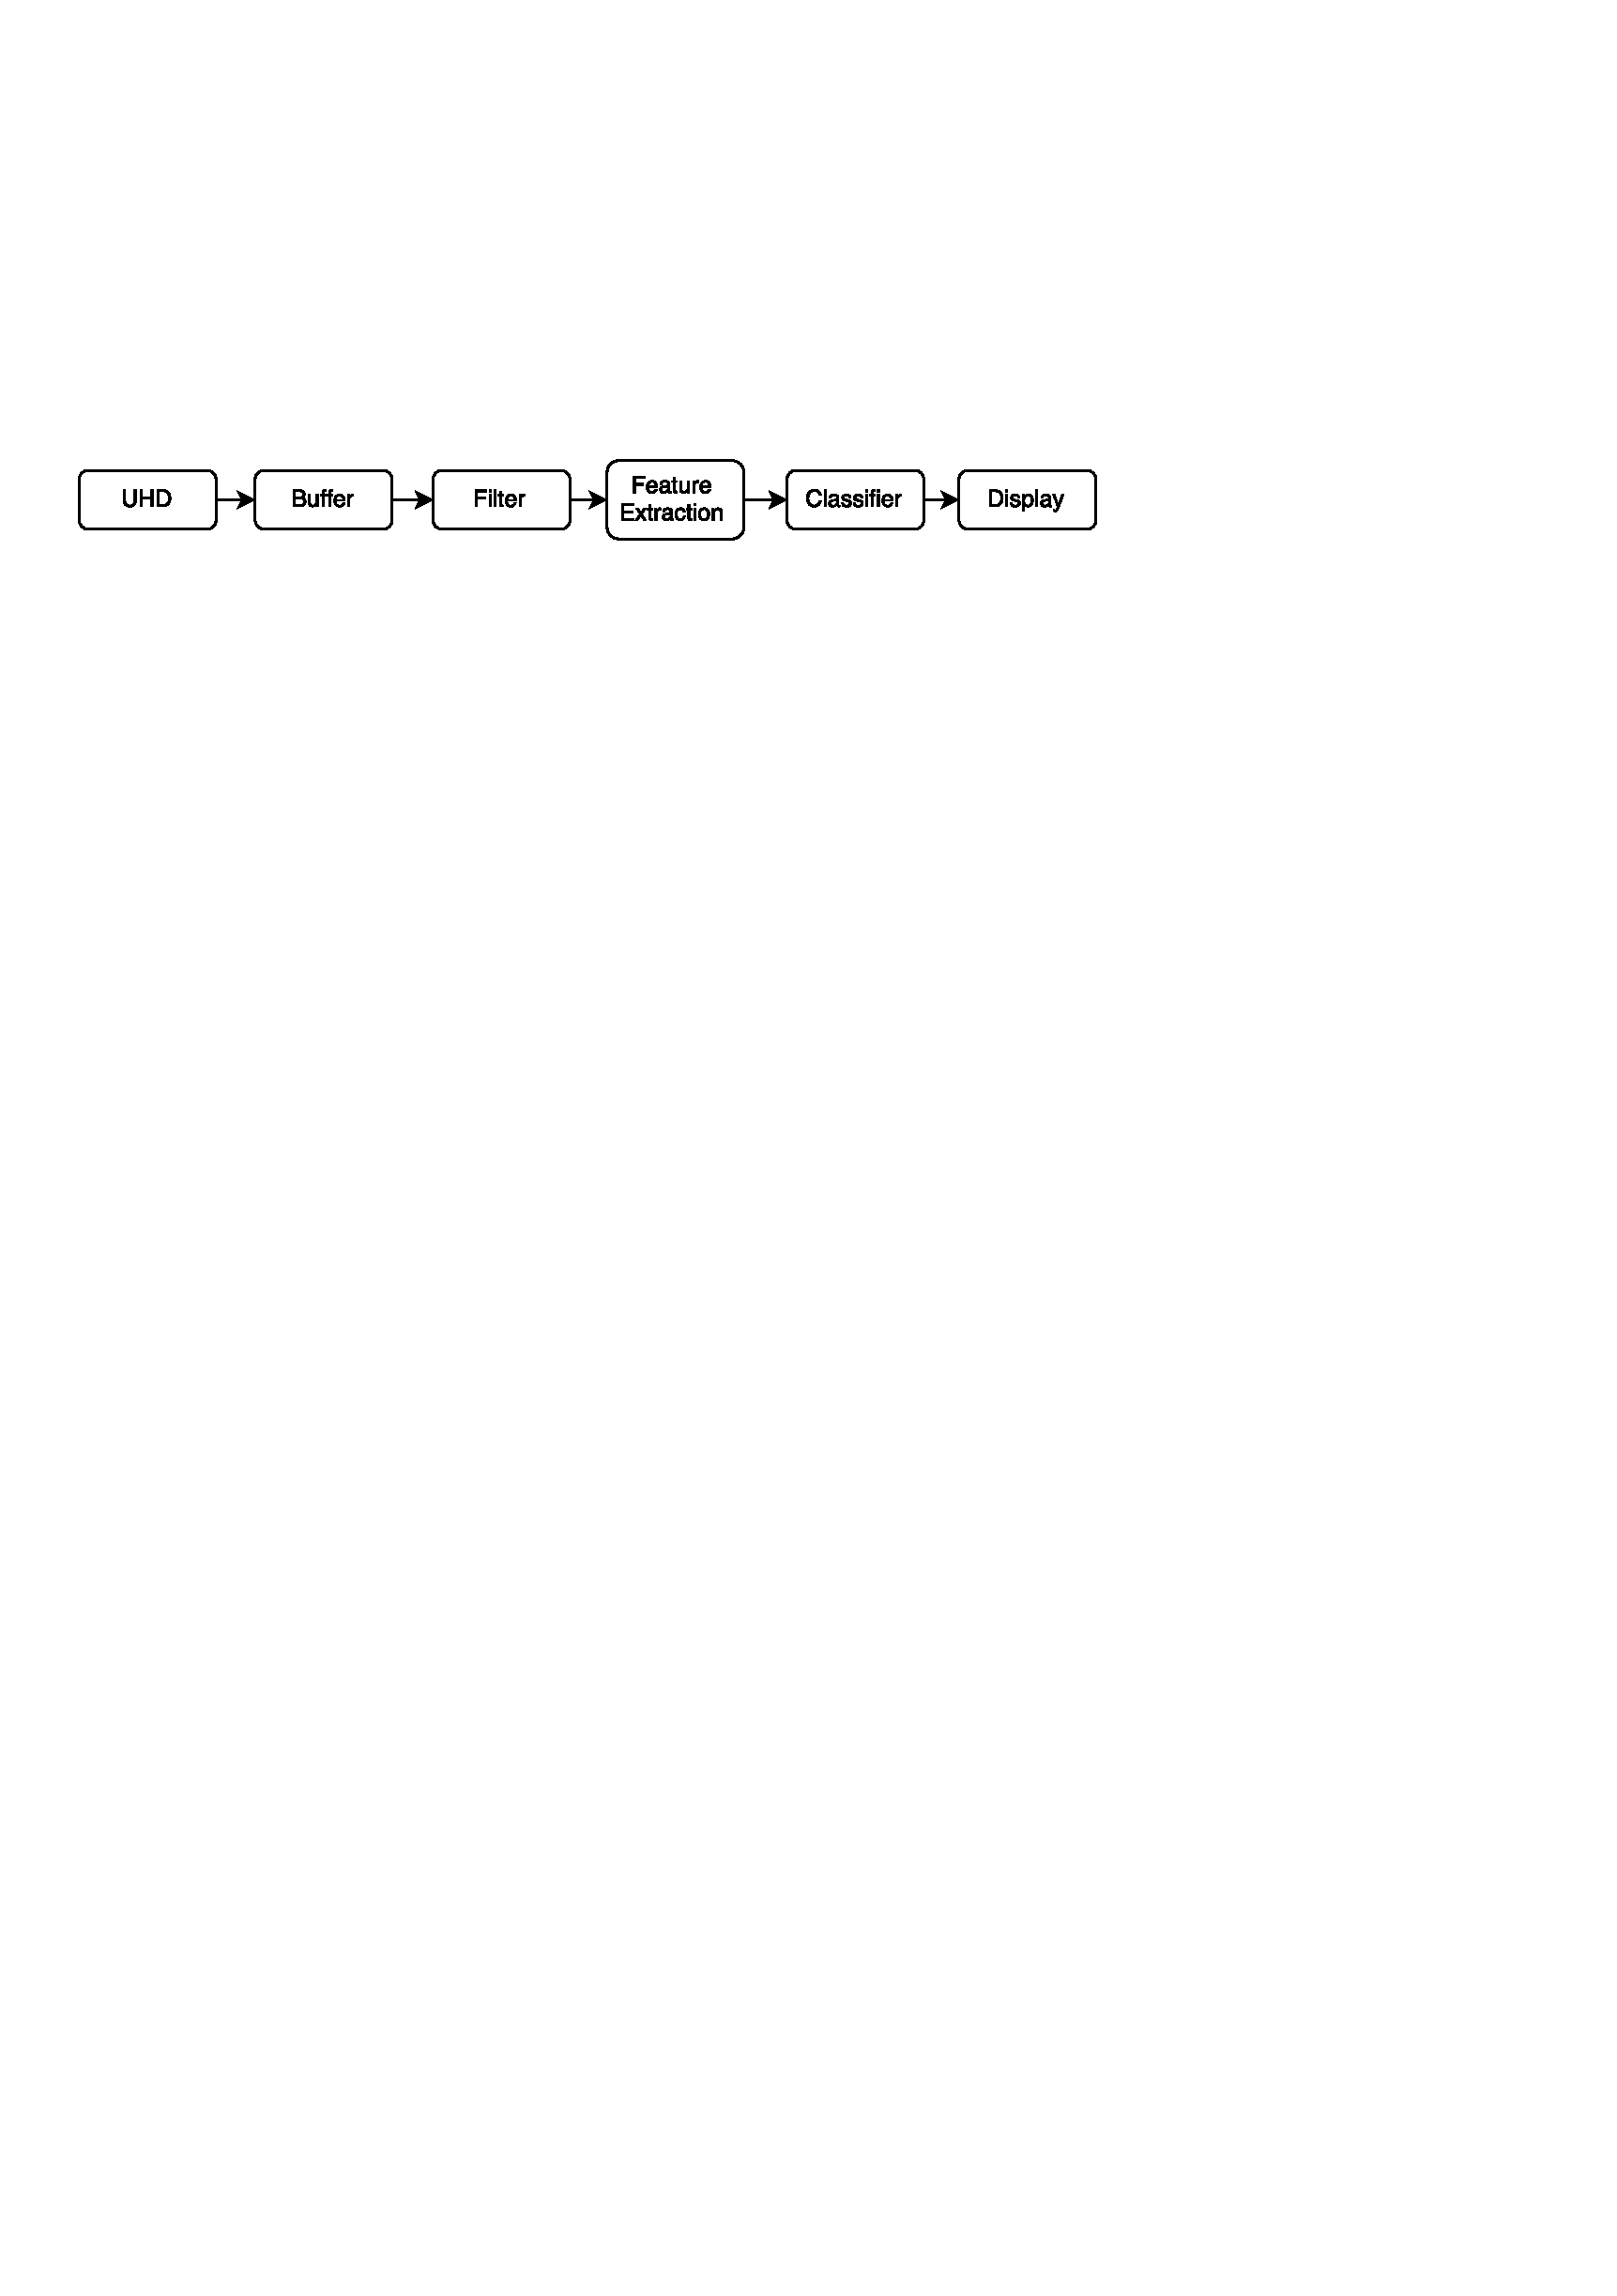
\includegraphics[trim=1.2cm 31.5cm 9cm 8cm, clip=true,width=0.5\textwidth]{small.pdf}
				\caption{Modulation Classification Algorithm Overview.}
				\label{fig:sw_overview}
			\end{figure}
		\subsubsection{Libraries and API's}

		\subsubsection{Build System}

			% Cmake because easy, also can be compiled on windows (probably UHD issue, though)

	\subsection{Feature Extraction Functions}
	\label{subsec:feature_extract}

	\subsection{Signal Filtering}

	\subsection{Classifier}

\section{PROPOSED TESTING PROCEDURE}
	\subsection{Functional Testing}
		% Evaluate system with generated signals
		% See how well it fares with different number of samples
		% Signal to noise ratio
	\subsection{Practical Testing}
		% correlate real world results with simulation
		% Don't make a new program, just use GNURadio companion to make signals to classify
\section{PRELIMINARY RESULTS}
	\begin{figure*}[!h]
		\centering
		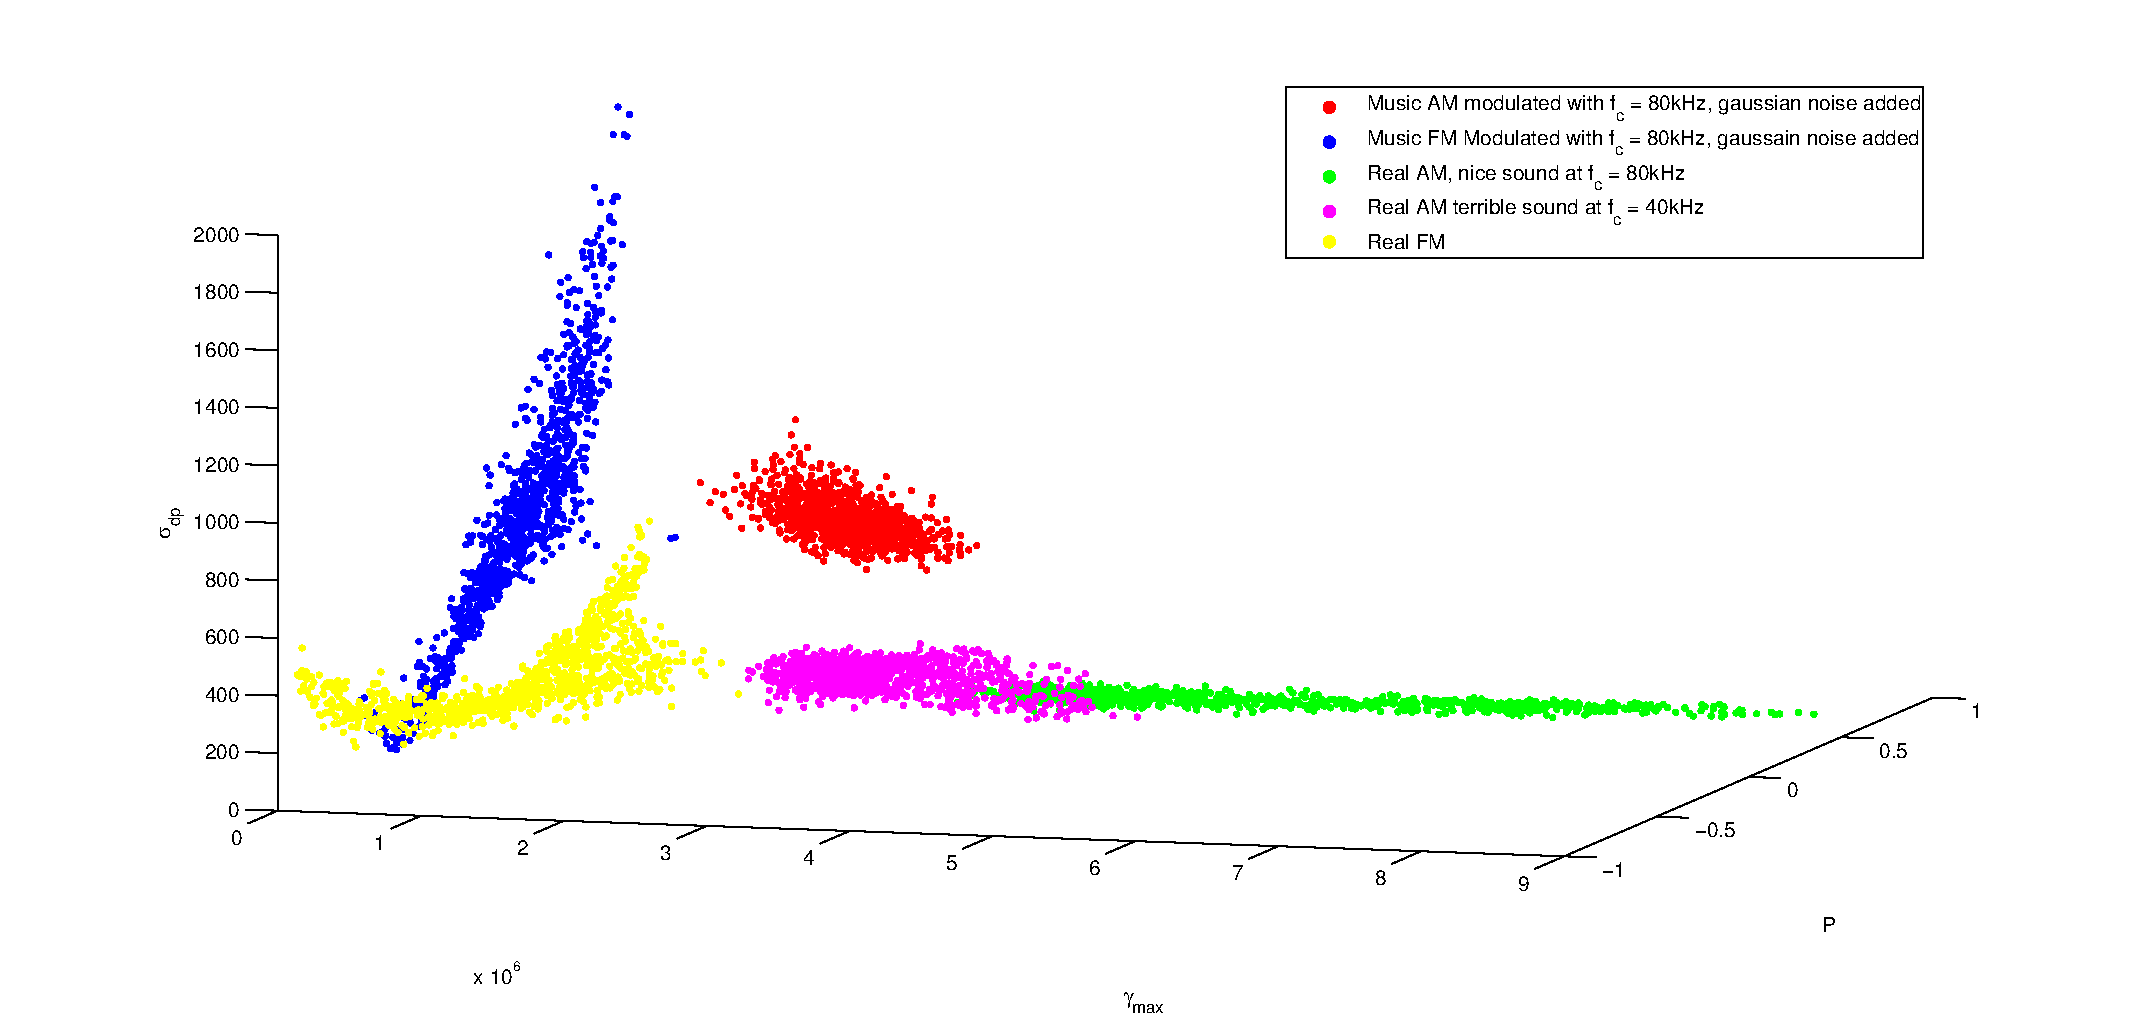
\includegraphics[width=1.1\textwidth]{plot0-eps-converted-to.pdf}
		\caption{Plot of $\sigma_{dp}$ vs. $\gamma_{max}$ vs. $P$ for various AM and FM signals}
		\label{fig:plot0}
	\end{figure*}
\section{CONCLUSION AND RECOMMENDATIONS}


\bibliographystyle{witseie}
\bibliography{prelim}
\end{document}
